% XeLaTeX + ctex 中文支持
\documentclass[UTF8,a4paper,10pt,oneside]{ctexart}

% ---------- 页面与基础 ----------
\usepackage{geometry} % 页面尺寸与页边距设置
\geometry{margin=2.5cm}
\usepackage{indentfirst} % 使章节后的首段缩进
\setlength{\parindent}{2em}
\usepackage{placeins} % 提供 \FloatBarrier 控制浮动体位置

% ---------- 数学与公式 ----------
\usepackage{amsmath,amssymb} % 高级数学公式环境与数学符号

% ---------- 图形与颜色 ----------
\usepackage[table]{xcolor} % 颜色支持（含表格着色）
\usepackage{graphicx} % 插入图片命令 \includegraphics
\usepackage{tikz} % 矢量绘图，配合 pgfplots 使用
\usetikzlibrary{positioning, calc, shapes.geometric, arrows.meta, backgrounds, external, fit} % TikZ 常用库

% ---------- 表格 ----------
\usepackage{booktabs} % 专业表格线命令（\toprule/\midrule/\bottomrule）
\usepackage{tabularx} % 可伸缩列宽的表格环境
\usepackage{array} % 表格列格式增强
\usepackage{multirow} % 合并多行单元格
\usepackage{longtable} % 跨页长表格
\usepackage{colortbl} % 表格单元格背景色支持

% ---------- 列表、代码与文本 ----------
\usepackage{enumitem} % 列表定制（间距、标签等）
\usepackage{soul} % 文本高亮（\hl）和删除线等
\usepackage{listings} % 源代码高亮与代码块样式
%========================================
% Emoji support using twemojis (Vector SVGs)
%========================================
\usepackage{twemojis} % 将 emoji 渲染为矢量图（twemoji SVG）
\usepackage{alltt} % 类似 verbatim 但允许 LaTeX 命令展开（用于示例输出）
\usepackage{alltt}

\usepackage{subfiles} % 支持将章节作为独立子文件编译
\usepackage[numbers,sort&compress]{natbib} % 参考文献样式与引用压缩

% ---------- 图题与浮动 ----------
\usepackage{float} % 强制浮动体位置（H）参数
\usepackage{caption} % 自定义图表题注样式
\usepackage{subcaption} % 子图题注环境

% ---------- 其他常用工具 ----------
\usepackage{changelog} % 变更日志支持（项目文档用途）
\usepackage{tcolorbox} % 彩色盒子用于提示、示例等
\tcbuselibrary{skins,breakable} % tcolorbox 的扩展库
\usepackage{etoolbox} % 编程型宏工具集合
\usepackage{siunitx} % 物理量与单位格式化

% ---------- TODO 注释 ----------
% 默认使用页边 TODO，尽量不影响正文排版。
\usepackage[textsize=scriptsize]{todonotes} % 文档内待办注释（边注）
\setlength{\marginparwidth}{2.1cm}

% ---- TikZ 外部化缓存 (首次编译生成 PDF，后续直接复用，大幅提速) ----
% 编译时必须开启 -shell-escape（VSCode 配置已设置）
% 如需临时关闭缓存（调试用），注释下面两行并取消 \tikzexternaldisable 的注释
% prefix 只能是项目根目录下的相对路径（不含 out/ 前缀），
% 因为 xelatex 的 -output-directory=out 会让 openout 自动在前面加 out/，
% 若 prefix 也写 out/ 则变成 out/out/tikz-cache/ —— 路径叠加导致写入失败。
% .md5 文件写到 out/tikz-cache/（kpathsea 会把 out/ 加入搜索路径，读取正常）；
% 外部化子进程（无 -output-directory）将 PDF 写到项目根 tikz-cache/，\includegraphics 可直接找到。
\tikzexternalize[prefix=tikz-cache/]
%\tikzexternaldisable  % 取消注释可关闭外部化，回退到内联编译（调试用）

% ---- 修复 tcolorbox (skins+breakable) 与 TikZ external 的兼容性冲突 ----
% tcolorbox skins 库内部会创建 tikzpicture 用于绘制边框/背景；
% TikZ external 全局 hook 会拦截这些内部 tikzpicture，在 breakable 跨页时
% 导致 collect@until@end@tikzpicture 状态错乱（Extra \else / extra } 等连锁错误）。
% 解决方案：在每个 tcolorbox / personalnote 环境的开头/结尾禁用/启用外部化。
\AtBeginEnvironment{tcolorbox}{\tikzexternaldisable}
\AtEndEnvironment{tcolorbox}{\tikzexternalenable}
\AtBeginEnvironment{personalnote}{\tikzexternaldisable}
\AtEndEnvironment{personalnote}{\tikzexternalenable}
\AtBeginEnvironment{taskbox}{\tikzexternaldisable}
\AtEndEnvironment{taskbox}{\tikzexternalenable}

\definecolor{ieeeBlue}{RGB}{0, 83, 159}
\definecolor{ieeeRed}{RGB}{198, 38, 46}
\definecolor{ieeeGreen}{RGB}{0, 114, 41}
\definecolor{ieeeOrange}{RGB}{235, 110, 31}
\definecolor{ieeeGray}{RGB}{100, 100, 100}
\definecolor{darkGray}{RGB}{66, 66, 66}
\definecolor{lightGray}{RGB}{189, 189, 189}

% TODO 全局样式与便捷命令
\setuptodonotes{
  color=ieeeOrange!15,
  bordercolor=ieeeOrange,
  linecolor=ieeeOrange
}
% todonotes 内部依赖 TikZ；开启 externalize 时需临时禁用外部化，避免编译失败。
\let\origTodo\todo
\RenewDocumentCommand{\todo}{ O{} m }{%
  \tikzexternaldisable
  \origTodo[#1]{#2}%
  \tikzexternalenable
}
\newcommand{\todoinline}[1]{\todo[inline,color=ieeeOrange!12]{#1}}

\usepackage{pgfplots} % 基于 TikZ 的函数与数据绘图
\pgfplotsset{compat=1.18}


% ctex 设置，确保各级标题缩进符合中文规范
\ctexset{
  paragraph/indent = 2em,
  subparagraph/indent = 2em,
}



% 链接相关宏包建议放在导言区靠后位置
\usepackage{hyperref}
\hypersetup{
  colorlinks=true,
  linkcolor=blue,
  urlcolor=blue,
  pdftitle={知识库文档},
  pdfauthor={葛良晨}
}

\lstdefinelanguage{riscv-asm}{
  morekeywords={add, addi, sub, sll, slli, srl, srli, sra, srai, and, andi, or, ori, xor, xori, slt, slti, sltu, sltiu,
    beq, bne, blt, bge, bltu, bgeu, jal, jalr, lui, auipc, lw, lh, lb, lhu, lbu, sw, sh, sb,
    csrr, csrw, csrrs, csrrc, csrrwi, csrrsi, csrrci, mret, ecall, ebreak, wfi, nop, ret, call, j, li, la, mv,
    .text, .data, .bss, .rodata, .section, .global, .globl, .align, .file, .type, .size, .word, .half, .byte, .asciz},
  morecomment=[l]{\#},
  morecomment=[l]{;},
  morestring=[b]",
  sensitive=true
}

\lstdefinelanguage{SystemVerilog}{
  morekeywords={
    always_comb, always_ff, always_latch, assert, assume, automatic, begin, end, case, endcase,
    class, endclass, clocking, endclocking, constraint, endconstraint, cover, covergroup, endgroup,
    default, disable, do, else, endfunction, endmodule, endpackage, endprogram, endtask, enum,
    export, extends, final, for, foreach, fork, join, join_any, join_none, function, generate,
    endgenerate, genvar, if, import, inside, interface, endinterface, localparam, logic, modport,
    module, new, package, program, protected, rand, randc, randcase, randsequence, ref, return,
    sequence, endsequence, struct, task, typedef, union, unique, unique0, virtual, void, wait, while,
    with
  },
  morecomment=[l]{//},
  morecomment=[s]{/*}{*/},
  morestring=[b]",
  sensitive=true
}

\lstset{
  basicstyle=\ttfamily\small,
  frame=single,
  breaklines=true,
  keywordstyle=\color{blue},
  commentstyle=\color{teal},
  stringstyle=\color{red!70!black}
}

% ---------- 自定义行内代码样式 ----------
\definecolor{codebg}{RGB}{230, 230, 230}
% 定义新命令 \code，避免直接修改 \texttt 导致系统崩溃
\newcommand{\code}[1]{\colorbox{codebg}{\ttfamily #1}}

% 保持 tcolorbox 的兼容性设置
\tcbset{shield externalize}





\title{RISC-V 技术文档 Demo}
\author{葛良晨}
\date{\today}

% 自定义个人总结环境
\newtcolorbox{personalnote}[1][]{
  colback=yellow!10,
  colframe=yellow!70!black,
  fonttitle=\bfseries,
  title=个人总结,
  breakable,
  enhanced,
  before upper={\setlength{\parindent}{2em}},
  #1
}

% 自定义待办事项环境
\newtcolorbox{taskbox}[1][]{
  colback=blue!5,
  colframe=blue!60!cyan!70!black,
  fonttitle=\bfseries,
  title=待办事项,
  breakable,
  enhanced,
  before upper={\setlength{\parindent}{2em}},
  #1
}

% 自定义妙妙想法彩框
\newtcolorbox{ideabox}[1][]{
  colback=purple!8!white,
  colframe=purple!60!black,
  fonttitle=\bfseries,
  title=✨ 妙妙想法,
  breakable,
  enhanced,
  before upper={\setlength{\parindent}{2em}},
  #1
}




\title{LLM 部署研究与资源安排}
\author{IC 设计部 内网研究}
\date{2026-05-17}

\begin{document}
\maketitle

% ======================================================================
% 第一章：LLM 本地部署的底层原理
% ======================================================================

\section{LLM 本地部署的底层原理}

在讨论"用什么硬件、选什么模型"之前，必须先理解 LLM 推理系统在物理层面到底发生了什么。
否则很容易陷入"看别人说 4090 能跑 70B 模型就行"的误区——能跑和能用之间，差了一整个工程体系。

\subsection{LLM 推理系统的基本组成}

一个 LLM 推理系统由以下核心组件构成：

\subsubsection{模型权重（Model Weights）}

Transformer 模型的"知识"以浮点数矩阵的形式存储。一个 7B（70亿参数）的模型，如果用 FP16（半精度浮点，每个参数 2 字节）存储，仅权重文件就约占 $7 \times 10^9 \times 2 \text{ bytes} = 14\text{ GB}$。

这是静态的、必须加载到显存中的部分。权重大小直接决定了显存的"底价"。

\subsubsection{Tokenizer}

Tokenizer 是将自然语言（或代码）转换为模型能理解的 token ID 序列的组件。它不是"简单的字符串切割"，而是基于 BPE（Byte Pair Encoding）或 SentencePiece 等算法的子词分割。

一个中文字符通常对应 1--3 个 token；一段英文单词也类似。IC 设计中的 Verilog 关键字、信号名、参数名会被切分成若干 token。Tokenizer 的质量直接影响模型对代码的理解能力——如果关键 Verilog 语法被切得太碎，模型对代码结构的感知就会退化。

\subsubsection{KV Cache}

KV Cache 是 Transformer 推理中最关键也最占内存的动态结构。其本质是：在自回归生成过程中，每个已生成的 token 的 Key 和 Value 矩阵被缓存下来，避免每次生成新 token 时重新计算所有历史 token 的 Attention。

KV Cache 的大小与以下因素成正比：
\begin{itemize}
    \item 层数（layers）
    \item 注意力头数（attention heads）
    \item 每头维度（head dimension）
    \item 上下文长度（context length）
    \item 精度（FP16/INT8 等）
\end{itemize}

一个粗略的经验公式：对于典型 7B 模型（32层，32头，128维/头），FP16 精度下，每 1K token 的 KV Cache 约为：
\[
2 \times 32 \text{ layers} \times 32 \text{ heads} \times 128 \text{ dim} \times 2 \text{ bytes} \times 1024 \text{ tokens} \approx 512\text{ MB}
\]
即大约 0.5 GB / 1K token。如果上下文扩到 128K，KV Cache 理论上是 $0.5 \times 128 = 64\text{ GB}$ ——这还没算权重本身。

\begin{figure}[htbp]
\centering
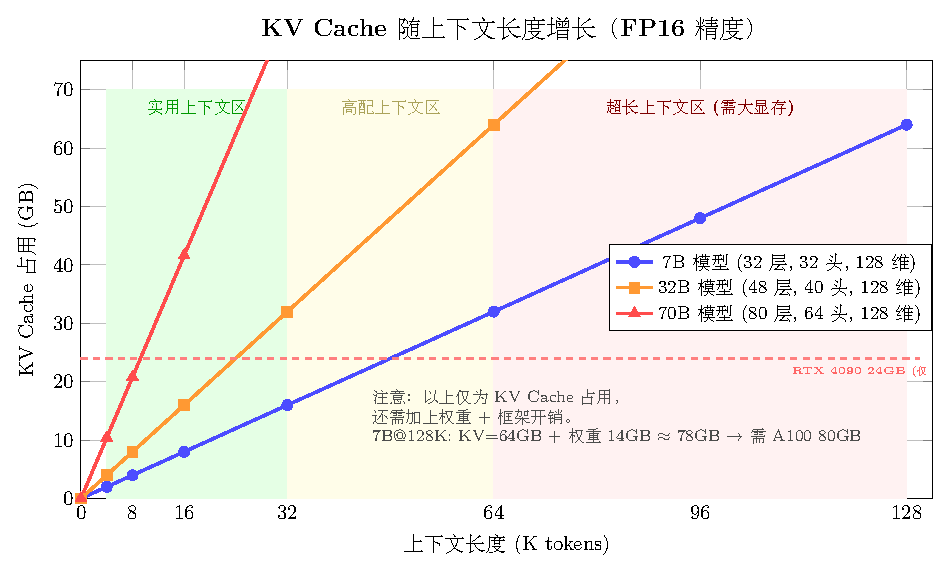
\includegraphics[width=0.95\textwidth]{figures/03-kvcache-vs-context.pdf}
\caption{KV Cache 随上下文长度增长曲线（FP16）。注意这仅为 KV Cache 部分，还需加上模型权重和框架开销。7B@128K 的 KV Cache 已达 64GB，足以吞没一张 RTX 4090 的全部显存。}
\end{figure}

这就是为什么"长上下文"本质上是用显存换来的，且是超线性代价。

\subsubsection{Context Window（上下文窗口）}

Context Window 是模型一次能"看到"的最大 token 数。常见的如 4K、8K、32K、128K、1M。窗口越大，模型能处理的连续文本越长，但 KV Cache 和 Attention 计算量也随之增长。

对于 IC 设计场景：如果想让模型读一个完整的 Verilog 模块（可能几千行），或者读一份 IP 数据手册（几十页 PDF），至少需要 32K 以上的上下文窗口，否则模型会在中途"遗忘"前面的内容。

\subsubsection{Embedding}

Embedding 是将 token ID 映射到高维向量空间的查找表。隐藏维度通常是 4096（7B 级）到 8192（70B 级）。Embedding 矩阵本身也占用显存，但相对权重矩阵而言较小。

\subsubsection{Attention 机制}

Attention 是 Transformer 的核心计算。在推理时，每个新生成的 token 需要对所有历史 token 做 Attention（通过 KV Cache 加速）。Attention 的计算复杂度与序列长度成二次方关系 $O(n^2)$ ——这是长上下文推理慢的根本原因之一。

Flash Attention（v1/v2/v3）通过分块计算和 IO 优化，大幅减少了 Attention 的显存访问量，是当前所有推理框架的标配。

\subsubsection{推理框架}

推理框架负责将模型文件加载到显存、管理 KV Cache、调度计算、处理并发请求。主流框架包括 llama.cpp、vLLM、SGLang、TensorRT-LLM 等（第 2 章详细对比）。

\subsection{GPU 显存到底在存什么}

很多人问"7B 模型需要多少显存"，但很少有人把显存的"账单"列清楚。以下是推理时 GPU 显存的实际占用分解：

\begin{enumerate}
    \item \textbf{模型权重}（静态，必须全部加载）

    \begin{itemize}
        \item FP16：参数量 $\times$ 2 bytes
        \item INT8：参数量 $\times$ 1 byte
        \item INT4：参数量 $\times$ 0.5 byte
    \end{itemize}

    \item \textbf{KV Cache}（动态，随上下文增长）

    \item \textbf{中间激活值}（推理框架的临时缓冲区，通常较小）

    \item \textbf{推理框架开销}（CUDA context、内核缓存等，通常 0.5--2 GB）
\end{enumerate}

一个完整的显存估算公式（工程经验）：

\begin{equation}
\begin{aligned}
\text{VRAM}_{\text{total}} \approx &\ \text{参数量} \times \text{每参数字节数} \\
                                  &+ 2 \times \text{层数} \times \text{头数} \times \text{头维度} \times 2 \times \text{上下文tokens} \\
                                  &+ 2\text{ GB (框架开销)}
\end{aligned}
\end{equation}

\begin{figure}[htbp]
\centering
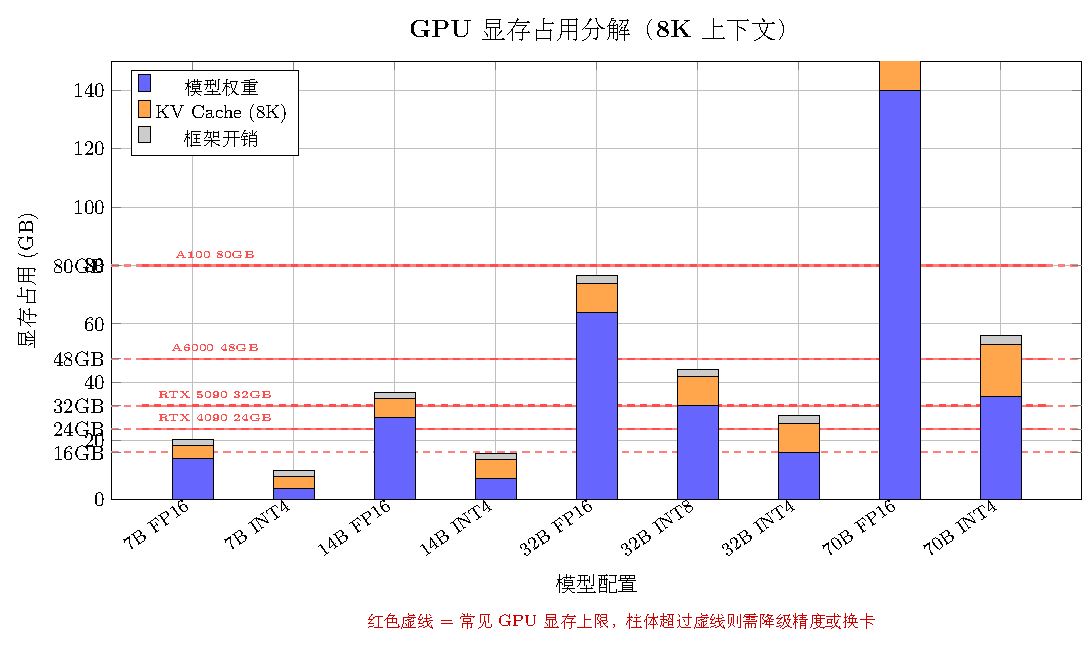
\includegraphics[width=0.95\textwidth]{figures/01-gpu-vram-breakdown.pdf}
\caption{GPU 显存占用分解（8K 上下文）。红色虚线为常见 GPU 显存上限，柱体超过虚线则需降低精度或更换 GPU。}
\end{figure}

举例：7B 模型，FP16，8K 上下文，32层，32头，128维：
\begin{itemize}
    \item 权重：$7 \times 10^9 \times 2 = 14\text{ GB}$
    \item KV Cache：$2 \times 32 \times 32 \times 128 \times 2 \times 8192 \div 10^9 \approx 4.3\text{ GB}$
    \item 框架开销：约 2 GB
    \item \textbf{总计：约 20--22 GB}
\end{itemize}

所以：\textbf{7B FP16 模型在 8K 上下文下，至少需要 24 GB 显存的 GPU（如 RTX 4090/3090）}。

\subsection{量化（Quantization）的本质}

量化是将模型参数从高精度（FP16/BF16）压缩到低精度（INT8/INT4），以减少显存占用和加速计算。

\subsubsection{常见精度格式}

\begin{itemize}
    \item \textbf{FP16}：半精度浮点，2 bytes/参数，标准推理精度
    \item \textbf{BF16}：Brain Float 16，与 FP16 同位宽但范围更大（与 FP32 指数位相同），在 A100/H100 上效率更高
    \item \textbf{INT8}：8位整数，1 byte/参数，通过校准（calibration）确定量化参数，精度损失通常 $\textless 1\%$
    \item \textbf{INT4}：4位整数，0.5 bytes/参数，需要更精细的量化策略（如 GPTQ、AWQ），精度损失约 1--3\%
    \item \textbf{GGUF}：llama.cpp 生态的文件格式，支持从 Q2\_K 到 Q8\_0 等多种量化级别，关键在于可以在 CPU+GPU 混合模式下运行
\end{itemize}

\subsubsection{量化对显存的实际影响}

以 32B 模型为例：

\begin{itemize}
    \item FP16：$32 \times 2 = 64\text{ GB}$ ——需要 A100 80GB 或双卡
    \item INT8：$32 \times 1 = 32\text{ GB}$ ——单张 A100 或 2$\times$RTX 4090
    \item INT4：$32 \times 0.5 = 16\text{ GB}$ ——单张 RTX 4090 即可
\end{itemize}

\textbf{但注意}：量化只压缩了权重部分！KV Cache 仍然是 FP16（大多数框架默认）。所以上下文长了之后，量化模型依然会面临 KV Cache 爆炸的问题。

\subsection{为什么 Prompt 越长越慢}

这个问题的本质有三层：

\subsubsection{第一层：Prefill 阶段}

输入 Prompt 时，模型需要一次性计算所有输入 token 的 Attention（双向/因果），这是计算密集型的。Prompt 越长，Prefill 时间越长。对于 32K token 的 Prompt，即使 H100 也需要数秒才能完成 Prefill。

\subsubsection{第二层：Decode 阶段}

生成每个新 token 时，需要与所有历史 token（Prompt + 已生成）做 Attention。KV Cache 越大，显存带宽压力越大。Decode 阶段是\textbf{显存带宽瓶颈}而非算力瓶颈。

\subsubsection{第三层：Attention 的二次方复杂度}

标准的因果 Attention 复杂度是 $O(L^2)$（$L$ 为序列长度）。Flash Attention 将其优化到 $O(L)$ 的显存访问，但计算量仍是 $O(L^2)$。

\subsection{推理瓶颈分析}

\subsubsection{算力 vs. 显存带宽}

对于 LLM 推理的 Decode 阶段（生成每个 token），\textbf{瓶颈几乎总是显存带宽，而非算力}。

原因：每次生成一个 token，需要从显存中读取全部权重（如 7B FP16 的 14 GB），做一次矩阵乘法（计算量相对很小），然后写入 KV Cache。整个过程的瓶颈在于这 14 GB 数据从 HBM 传输到计算单元的速度。

这就是为什么：
\begin{itemize}
    \item H100（3.35 TB/s 显存带宽）比 A100（2 TB/s）推理更快，尽管算力差距没那么大
    \item RTX 4090（1 TB/s 带宽）虽然算力不低，但推理大模型时带宽明显不够
    \item Apple Silicon M2 Ultra（800 GB/s 统一内存带宽）在推理大模型时表现不错，就是因为带宽大
\end{itemize}

\begin{figure}[htbp]
\centering
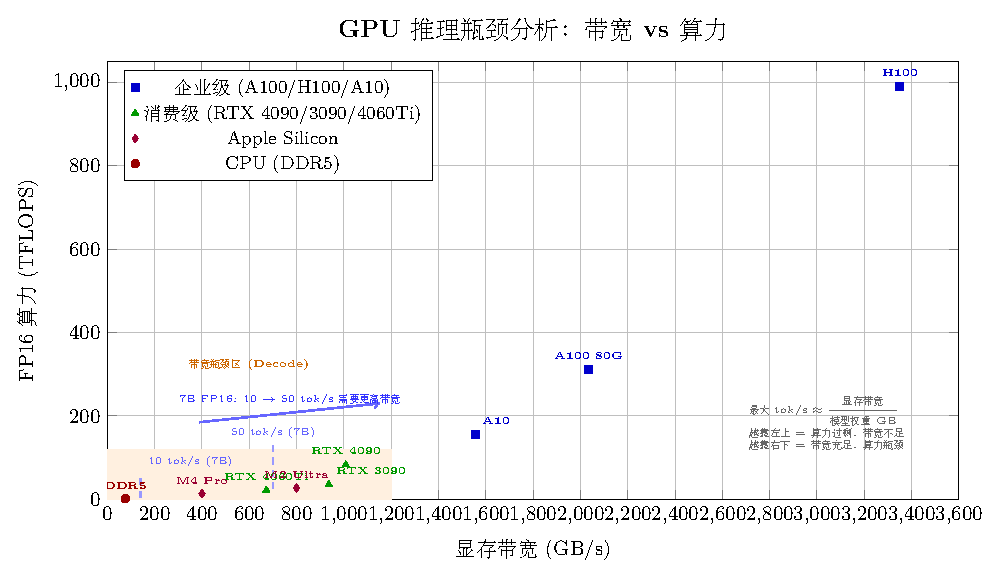
\includegraphics[width=0.95\textwidth]{figures/02-inference-bottleneck.pdf}
\caption{GPU 推理瓶颈分析：显存带宽 vs FP16 算力。左下角橙色区域为 Decode 阶段的带宽瓶颈区——大部分消费级 GPU 处于此区域。越靠左上意味着算力过剩而带宽不足，这正是 LLM 推理的典型特征。}
\end{figure}

\subsubsection{CPU-Only 为什么慢}

CPU 推理慢的根本原因是\textbf{内存带宽}。DDR5 双通道约 50--80 GB/s，而 RTX 4090 的显存带宽是 1008 GB/s，差距约 15--20 倍。

7B FP16 模型在 CPU 上推理：
\[
\text{理论最大速度} \approx \frac{80\text{ GB/s}}{14\text{ GB}} \approx 5.7\text{ tokens/s}
\]
实际由于 cache miss、操作系统开销，通常只有 2--5 tokens/s。

在 GPU 上：
\[
\text{理论最大速度} \approx \frac{1000\text{ GB/s}}{14\text{ GB}} \approx 71\text{ tokens/s}
\]
实际约 30--50 tokens/s。

\subsubsection{Apple Silicon 为什么适合个人 LLM}

Apple M 系列芯片的"统一内存架构"意味着 CPU 和 GPU 共享同一块高带宽内存。M2 Ultra 拥有 800 GB/s 的统一内存带宽，且最高可配置 192 GB。

这意味着：
\begin{itemize}
    \item 不需要通过 PCIe 在 CPU 和 GPU 之间搬运数据（这往往是多卡推理的瓶颈）
    \item 可以加载非常大的模型（如 70B Q4），利用全部统一内存
    \item 功耗极低（M2 Ultra 整机约 60--100W，而一张 A100 就 400W）
\end{itemize}

但限制也很明显：
\begin{itemize}
    \item 绝对算力远不如数据中心 GPU
    \item 不支持 CUDA 生态（Metal 的 ML 框架要弱很多）
    \item 多机扩展困难
    \item 不适合高并发服务
\end{itemize}

\textbf{结论：Apple Silicon 是个人本地 LLM 的甜点，但在企业服务场景中不适合。}

\subsubsection{企业级 GPU vs. 消费级 GPU}

\begin{table}[htbp]
\centering
\caption{企业级 vs 消费级 GPU 关键差异}
\begin{tabular}{p{2cm}p{5.5cm}p{3.5cm}}
\hline
\textbf{维度} & \textbf{企业级 (A100/H100)} & \textbf{消费级 (RTX 4090)} \\
\hline
显存 & 40/80 GB HBM2e/HBM3 & 24 GB GDDR6X \\
显存带宽 & 2--3.35 TB/s & 1 TB/s \\
NVLink & 有（多卡互联） & 无 \\
FP64/FP32 & 强 & 弱（被阉割） \\
ECC & 有 & 无 \\
功耗 & 300--700W & 450W \\
虚拟化 & MIG 支持 & 无 \\
保修/散热 & 数据中心级 & 消费级 \\
价格 & \$15K--\$35K & \$1.6K \\
\hline
\end{tabular}
\end{table}

\textbf{核心差异}：企业级 GPU 的壁垒不在算力，而在于显存容量+显存带宽+多卡互联+ECC+虚拟化。对于企业部署 LLM，如果不需要多卡互联和高并发，RTX 4090/5090 可能是性价比更高的选择——但需要接受消费级显卡的散热、稳定性和无 ECC 的风险。

\subsection{能跑 vs. 好用：工程鸿沟}

这是本报告最重要的概念之一。以下是一个真实对比：

\begin{table}[htbp]
\centering
\caption{能跑 vs. 好用}
\begin{tabular}{p{2cm}p{4cm}p{5cm}}
\hline
\textbf{维度} & \textbf{能跑（Demo）} & \textbf{好用（Production）} \\
\hline
响应速度 & 5--10 s/token（不可用）& $\textgreater$20 tokens/s（流畅）\\
并发 & 1 人独占 & 5--20 人同时使用 \\
上下文 & 2K--4K & 32K--128K \\
可靠性 & 偶尔 OOM 崩溃 & 7$\times$24 稳定 \\
量化 & Q4（有明显退化）& Q8 或 FP16 \\
RAG & 无或简陋 & 完整检索链路 \\
监控 & 无 & GPU 利用率、延迟 P50/P99 \\
\hline
\end{tabular}
\end{table}

很多开源项目展示的"7B 模型在树莓派上运行"属于"能跑"，但它可能每秒只生成 0.5 个 token——工程师不可能用它来提高效率。

\section{主流本地部署方案调研}

\subsection{模型选型分析}

\subsubsection{Llama 系列（Meta）}

Llama 3.1/3.2 系列是当前开源社区的事实基准。8B 模型在代码理解上表现不错，70B 模型接近 GPT-4 水平。Llama 系列的优势在于生态最成熟（vLLM、Ollama、llama.cpp 第一时间适配），社区活跃，但中文能力偏弱（Llama 3.1 后有所改善）。对 IC 设计场景：英文文档/代码场景完全可用，中文技术文档可能需要补充微调。

\subsubsection{Qwen 系列（阿里）}

Qwen 2.5 系列的中文能力在开源模型中领先，且代码能力（Qwen2.5-Coder）在 HumanEval 等基准上表现优异。有 0.5B/1.5B/7B/14B/32B/72B 多个尺寸。对 IC 设计场景：如果团队内部中文沟通较多、需要处理中文 Spec 和文档，Qwen 是首选。Qwen2.5-Coder-32B 是当前代码开源模型的最强之一。

\subsubsection{DeepSeek 系列（DeepSeek）}

DeepSeek-V2/V3 以 MoE（Mixture of Experts）架构著称，在极低推理成本下达到顶级性能。DeepSeek-Coder-V2 在代码任务上表现突出。但 DeepSeek 系列模型较大（236B 总参数，21B 激活参数/V2），本地部署门槛较高。对 IC 设计场景：如果硬件资源充足，DeepSeek 的代码理解和生成能力非常强，尤其适合 SystemVerilog/UVM 等复杂代码场景。

\subsubsection{Mistral / Mixtral}

Mistral 7B 和 Mixtral 8$\times$7B（MoE，总 47B，激活 13B）在欧洲社区使用广泛。英文代码能力扎实，但中文较弱。Mixtral 的 MoE 架构在推理时只激活部分参数，效率高，适合中等硬件。

\subsubsection{CodeLlama / StarCoder / DeepSeek-Coder}

这些是专门的代码模型。StarCoder2 有 3B/7B/15B 多个尺寸，训练数据来自 The Stack v2（大量 GitHub 代码），包含 Verilog、SystemVerilog、Tcl 等硬件描述语言的训练数据。对 IC 设计场景：专门代码模型在 Verilog 补全、testbench 生成上优于通用模型，但缺乏对设计约束（时序、面积、功耗）的深层理解。

\subsubsection{Gemma 系列（Google）}

Gemma 2 9B/27B 在同等参数规模下性能出色。但 Gemma 系列的使用条款有商业限制，企业需要注意合规问题。

\subsubsection{模型推荐矩阵}

\begin{table}[htbp]
\centering
\caption{IC 设计场景模型推荐}
\begin{tabular}{p{2.5cm}p{3.10cm}p{3.2cm}p{3.5cm}p{1.8cm}}
\hline
\textbf{场景} & \textbf{推荐模型} & \textbf{理由} & \textbf{备选} & \textbf{最小显存} \\
\hline
代码补全 & Qwen2.5-Coder-7B & 代码能力好，轻量 & DeepSeek-Coder-6.7B & 16 GB \\
代码理解/审查 & Qwen2.5-Coder-32B & 32B 是代码理解甜点 & DeepSeek-Coder-V2 & 24 GB (Q4) \\
中文文档/RAG & Qwen2.5-14B & 中文最好 & Qwen2.5-32B & 16 GB (Q4) \\
通用助手 & Llama-3.1-8B & 生态最好 & Mistral-7B & 16 GB \\
最高代码质量 & Qwen2.5-Coder-32B/DeepSeek-Coder-V2 & 顶级 & — & 40 GB+ (FP16) \\
\hline
\end{tabular}
\end{table}

\subsection{推理框架全面对比}

\subsubsection{Ollama}

Ollama 是目前最易用的本地 LLM 工具。它封装了 llama.cpp，提供了类似 Docker 的使用体验（ollama pull、ollama run），自动管理模型下载、量化版本切换、GPU 加速。适合个人和极小型团队快速体验，但不适合多用户并发服务——它的服务模型是单请求队列的，且缺乏生产级的监控和负载均衡。

\textbf{适用场景：个人实验、3--5 人小团队内部快速验证。}

\subsubsection{llama.cpp}

llama.cpp 是 C/C++ 实现的 LLM 推理引擎，是本地 LLM 推理的基石。其核心贡献是 GGUF 格式和 CPU-GPU 混合推理。llama.cpp 在 Apple Silicon 上通过 Metal 加速表现优异，在 NVIDIA GPU 上通过 CUDA 加速也很成熟。

关键能力：
\begin{itemize}
    \item 任意量化级别（Q2\_K 到 Q8\_0，甚至 FP16）
    \item CPU-only 模式（虽慢但能跑）
    \item CPU+GPU 混合（部分层在 GPU，部分在 CPU）
    \item 支持多 GPU（但不支持张量并行，只是模型拆分）
\end{itemize}

\textbf{适用场景：几乎所有本地部署的基础层，个人和小团队的首选推理引擎。}

\subsubsection{vLLM}

vLLM 是目前生产环境中最主流的开源推理框架。其核心创新是 PagedAttention——将 KV Cache 像操作系统管理虚拟内存一样分页管理，大幅减少了显存碎片和浪费。

vLLM 的关键能力：
\begin{itemize}
    \item \textbf{连续批处理（Continuous Batching）}：多个请求可以在同一批次中动态进出，显存利用率极高
    \item \textbf{PagedAttention}：KV Cache 利用率从通常的 20--40\% 提升到接近 100\%
    \item \textbf{OpenAI API 兼容}：直接替换 OpenAI SDK 的 base\_url
    \item \textbf{张量并行}：支持多 GPU 拆分模型（如 2$\times$RTX 4090 跑 70B Q4）
    \item \textbf{前缀缓存}：相同系统提示词自动复用 KV Cache
\end{itemize}

\textbf{适用场景：企业级多用户部署。当前生产环境首选。}

\subsubsection{SGLang}

SGLang 是 Stanford 等团队推出的新一代推理框架，在 vLLM 的基础上加入了结构化生成（如 JSON 模式约束）和 RadixAttention（比 PagedAttention 更高效的前缀缓存）。在部分基准上比 vLLM 快 2--5$\times$。

\textbf{适用场景：对推理延迟敏感的生产环境，特别是需要结构化输出（如 Agent 的 Tool Calling）的场景。}

\subsubsection{TensorRT-LLM（NVIDIA）}

NVIDIA 官方的推理优化框架，利用 TensorRT 的图优化、算子融合、INT8/INT4 量化（通过 TensorRT Model Optimizer），在 NVIDIA GPU 上达到极致推理性能。

优势：性能天花板最高（相比 vLLM 可提升 2--4$\times$），支持 FP8（H100），支持 In-flight Batching。

劣势：部署复杂（需要模型转换、编写 Batching 配置），模型支持不如 vLLM 广泛，依赖 NVIDIA 生态（非 NVIDIA GPU 无法使用）。

\textbf{适用场景：对性能有极致要求、使用 NVIDIA 企业级 GPU 的生产环境。}

\subsubsection{HuggingFace TGI（Text Generation Inference）}

HuggingFace 官方的推理服务，功能与 vLLM 类似（连续批处理、张量并行、量化），但生态更偏向 HuggingFace Hub 的模型。HuggingFace 自身生产环境使用 TGI，成熟度有保障。

\textbf{适用场景：深度绑定 HuggingFace 生态的团队。}

\subsubsection{LM Studio / Open WebUI / AnythingLLM / text-generation-webui}

这些是"前端工具"，不是推理引擎。它们通常对接 Ollama 或 llama.cpp 的后端，提供聊天界面、文件上传、RAG 等。

\begin{itemize}
    \item \textbf{LM Studio}：图形化下载模型、管理本地推理，极简体验，适合个人
    \item \textbf{Open WebUI}：类 ChatGPT 的 Web 界面，支持 Ollama/OpenAI 后端，适合团队共享
    \item \textbf{AnythingLLM}：内置 RAG 的 LLM 客户端，适合构建知识库
    \item \textbf{text-generation-webui (oobabooga)}：功能最全的本地 WebUI，支持几乎所有后端
\end{itemize}

\subsubsection{框架推荐矩阵}

\begin{table}[htbp]
\centering
\caption{推理框架选型推荐}
\begin{tabular}{p{2.2cm}p{4cm}p{2.5cm}p{4.5cm}}
\hline
\textbf{场景} & \textbf{推荐框架} & \textbf{理由} & \textbf{备选} \\
\hline
个人实验 & Ollama + Open WebUI & 5 分钟上手 & LM Studio \\
3--10 人团队 & vLLM + Open WebUI & 并发支持好 & Ollama（如果无并发需求）\\
生产部署 & vLLM 或 SGLang & 工业级稳定 & TensorRT-LLM（性能优先）\\
Apple Silicon & llama.cpp + Ollama & Metal 加速最好 & — \\
NVIDIA 多卡 & vLLM（张量并行） & 开箱即用 & TensorRT-LLM \\
\hline
\end{tabular}
\end{table}

\begin{figure}[htbp]
\centering
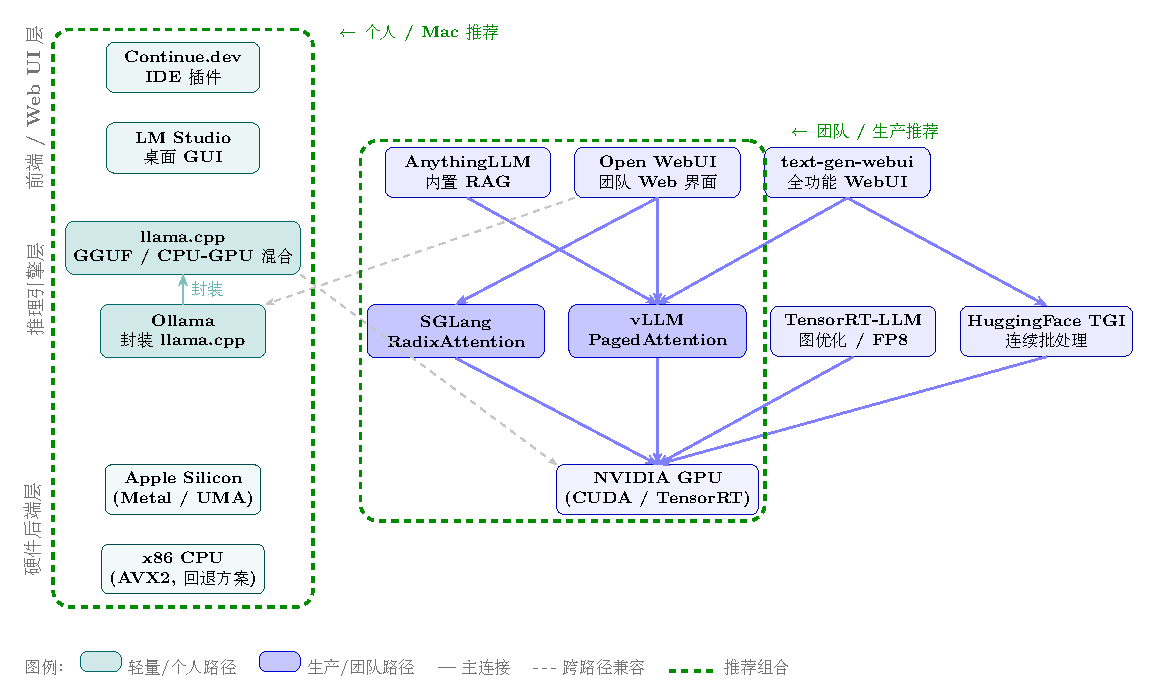
\includegraphics[width=0.95\textwidth]{figures/04-framework-ecosystem.pdf}
\caption{推理框架生态架构：前端层→推理引擎层→硬件后端层。绿色虚线标注推荐组合（Continue.dev + vLLM 或 Open WebUI + Ollama）。}
\end{figure}

% ======================================================================
% 第三章：最低资源验证可行性
% ======================================================================

\section{如果只是验证可行性，最低资源需要多少？}

这是初创公司最务实的问题：在投入真金白银之前，最少花多少钱能判断"这条路值不值得走"。

\subsection{分水岭：能启动 vs. 能用}

\begin{table}[htbp]
\centering
\caption{PoC 硬件分水岭}
\begin{tabular}{p{3.5cm}p{6.0cm}p{1.5cm}p{2.5cm}}
\hline
\textbf{级别} & \textbf{能启动} & \textbf{能用} & \textbf{推荐} \\
\hline
CPU-only & 任何 x86 服务器，32GB RAM，7B Q4，2--5 tok/s & 不可用 & 不推荐 \\
Mac Mini M4 Pro & 24GB 统一内存，7B Q4，15--25 tok/s & 勉强可用 & 个人实验 \\
Mac Studio M2 Ultra & 192GB，70B Q4，8--15 tok/s & 个人可用 & 太贵（¥40K+）\\
RTX 4060 Ti 16GB & 7B Q4，8K ctx & 单人勉强 & 低预算起步 \\
RTX 4090 24GB & 14B Q4 / 32B Q4，32K ctx，30--50 tok/s & \textbf{可用} & \textbf{甜点} \\
RTX 5090 32GB & 32B Q4 / 14B FP16，64K ctx & \textbf{好用} & 高性能甜点 \\
2$\times$RTX 4090 & 70B Q4，张量并行，32K ctx & 团队可用 & 团队起步 \\
A100 80GB & 70B FP16，128K ctx，高并发 & 生产就绪 & 正式部署 \\
\hline
\end{tabular}
\end{table}

\subsection{PoC 的三个层次}

\subsubsection{层次一：零成本体验（0 元，0 天）}

直接使用现有开发服务器（如果有 NVIDIA GPU 的话），或者用工程师的 MacBook Pro（M 系列，16GB+ 内存），安装 Ollama，拉取 Qwen2.5-Coder-7B-Q4\_K\_M。

\textbf{能做什么}：
\begin{itemize}
    \item 在 Ollama 的终端对话中体验代码补全
    \item 用 Continue.dev（VS Code 插件）对接 Ollama 做行内补全
    \item 感受一下"AI 写 Verilog"是什么效果
\end{itemize}

\textbf{不能做什么}：
\begin{itemize}
    \item 不能严肃评估对研发效率的提升
    \item 响应速度慢会让工程师失去兴趣（第一印象差）
    \item 小模型在复杂 IC 问题上会"胡说八道"
\end{itemize}

\textbf{结论：这只适合确认"这个方向有意思"，不能用于决策。}

\subsubsection{层次二：低成本 PoC（约 ¥15K，1--2 天）}

购买一张 RTX 4090 24GB（或使用已有显卡），装在一台有 64GB RAM + 2TB NVMe SSD 的 Linux 工作站上。Ubuntu 24.04 LTS + NVIDIA 驱动 + CUDA + Docker + vLLM + Open WebUI。

部署 Qwen2.5-Coder-32B-Q4\_K\_M（约 20GB 显存占用），32K 上下文。

\textbf{能做什么}：
\begin{itemize}
    \item 3--5 人同时使用，感受正常响应速度（20--40 tok/s）
    \item 测试代码补全、代码审查、文档问答
    \item 构建小型 RAG 知识库（内部 100--500 份文档）
    \item 评估模型在 Verilog/SystemVerilog 上的真实表现
\end{itemize}

\textbf{这是 PoC 的甜点方案。} 在这个配置上做 2--4 周的内部试用，足以决定是否值得投入正式部署。

\subsubsection{层次三：准生产 PoC（约 ¥60K--¥120K，1--2 周）}

2$\times$RTX 4090（或 RTX 5090）+ 128GB RAM + 4TB NVMe + Ubuntu 24.04。vLLM 张量并行部署 Qwen2.5-72B-Q4 或 DeepSeek-Coder-V2。

\textbf{能做什么}：
\begin{itemize}
    \item 10--20 人团队正常使用
    \item 128K 长上下文（读完整 IP 手册）
    \item 完整 RAG 系统
    \item Agent 实验（自动运行仿真、分析 log）
\end{itemize}

\subsection{Mac mini 是否够？}

坦白说：\textbf{对于企业 PoC，不推荐 Mac mini。}

理由：
\begin{itemize}
    \item M4 Pro Mac mini 最多 64GB 统一内存（约 ¥20K+），但这笔钱不如买一台二手 RTX 4090 工作站
    \item Metal 加速在 vLLM/SGLang 等生产框架中支持不完善
    \item 无法扩展到多卡/多机
    \item macOS 的 Docker 支持是虚拟机，有性能损耗
    \item 企业中最终还是 Linux + NVIDIA，PoC 阶段就应该用最终平台
\end{itemize}

唯一的例外：如果公司已经有 Mac Studio M2 Ultra 192GB 作为工程师的工作站，可以顺手在上面跑 PoC——但这只是"顺便用一下"，不是"为此购买"的理由。

\subsection{二手服务器是否值得？}

二手 NVIDIA V100 32GB 或 A100 40GB 在企业退役市场上流通，价格约为原价的 30--50\%。V100 32GB 二手约 ¥20K--¥30K，性价比不错。

\textbf{但需要注意}：
\begin{itemize}
    \item V100 不支持 BF16（只有 FP16），部分新模型可能不兼容
    \item 二手企业卡可能已经运行了 3--5 年，剩余寿命不确定
    \item 需要合适的服务器平台（PCIe 供电、散热、风扇噪音）
    \item 没有保修——如果坏了就是坏了
\end{itemize}

\textbf{结论：二手 V100 32GB 是预算紧张时的可行选择，但 RTX 4090 更推荐。}

\subsection{PoC 阶段的功耗与成本}

\begin{table}[htbp]
\centering
\caption{PoC 方案成本对比}
\begin{tabular}{p{3cm}p{1.5cm}p{1.5cm}p{1.5cm}p{2cm}p{1.5cm}}
\hline
\textbf{方案} & \textbf{硬件成本} & \textbf{功耗（空闲/满载）} & \textbf{月电费（¥0.8/kWh）} & \textbf{模型} & \textbf{速度} \\
\hline
MacBook Pro M4 Pro 24GB & ¥18K& 5W/30W & ¥17 & 7B Q4 & 15--20 t/s \\
RTX 4090 工作站 & ¥25K & 80W/500W & ¥288 & 32B Q4 & 30--50 t/s \\
2$\times$RTX 4090 & ¥40K & 120W/800W & ¥460 & 70B Q4 & 15--25 t/s \\
A100 80GB 二手 & ¥50K & 80W/400W & ¥230 & 70B FP16 & 40--60 t/s \\
\hline
\end{tabular}
\end{table}

注：电费按 24/7 运行计算。实际 PoC 阶段通常不是 24/7，成本更低。

% ======================================================================
% 第四章：IC 设计场景中的真实落地方式
% ======================================================================

\section{IC 设计场景中的真实落地方式}

这是本报告最核心的章节。我们不讲"AI 赋能"这样的空话，而是逐场景分析：LLM 到底能做什么、不能做什么、收益有多大、风险在哪里。

\begin{figure}[htbp]
\centering
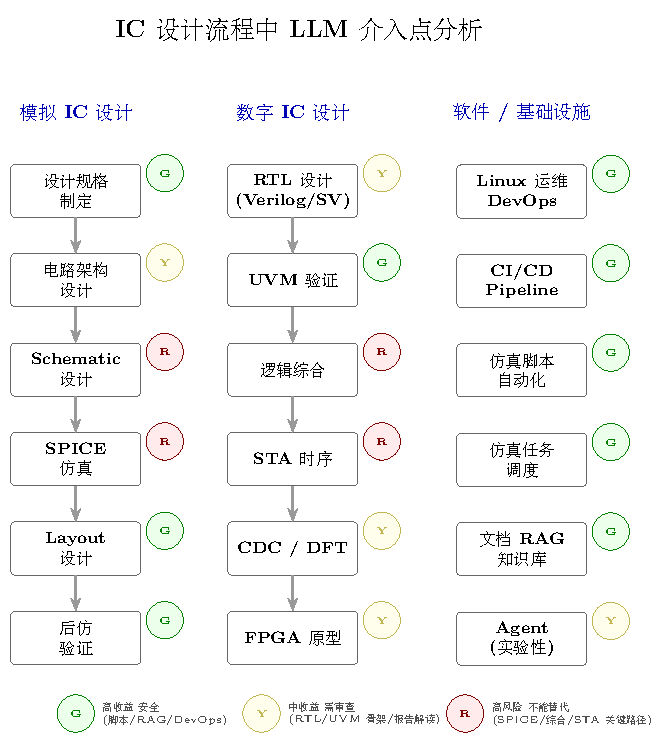
\includegraphics[width=0.95\textwidth]{figures/05-ic-flow-llm-intervention.pdf}
\caption{IC 设计流程中 LLM 介入点全景。绿色(G)=高收益安全区（脚本/RAG/DevOps），黄色(Y)=中收益需审查（RTL骨架/报告解读），红色(R)=高风险不能替代（SPICE/综合/STA关键路径）。}
\end{figure}

\subsection{模拟 IC 设计场景}

\subsubsection{电路阅读与理解}

\textbf{能做什么}：
\begin{itemize}
    \item 读网表（netlist），解释电路拓扑结构
    \item 识别常见结构：Bandgap、运放、比较器、LDO、偏置电路
    \item 解释器件尺寸选择的 trade-off（如"为什么输入对管用 10/0.18"）
    \item 翻译和总结电路设计文档
\end{itemize}

\textbf{局限}：
\begin{itemize}
    \item LLM 不理解物理——不知道 parasitic、mismatch、noise 的实际影响
    \item 对先进工艺节点（3nm/5nm）的特殊效应（如 DIBL、GIDL）缺乏深层理解
    \item 不能做真正的"电路分析"——那是 SPICE 的工作
\end{itemize}

\textbf{收益评级}：★★★☆☆（中等，辅助阅读有用，但不能替代工程师的判断）

\subsubsection{Bandgap / PLL / ADC/DAC / SerDes 设计}

\textbf{能做什么}：
\begin{itemize}
    \item 提供经典架构参考（如 Brokaw Bandgap、Type-II PLL、Pipeline ADC）
    \item 生成初始器件参数（如"设计一个 1.2V Bandgap，TC $\textless$ 20ppm/°C"）
    \item 解释设计公式和 trade-off
    \item 生成仿真 testbench 的骨架代码
\end{itemize}

\textbf{不能做什么（危险区域）}：
\begin{itemize}
    \item \textbf{不能替代 SPICE 仿真}——LLM 给出的参数只是"看起来合理"，必须在仿真器中验证
    \item \textbf{不了解具体工艺}——不同 foundry 的 PDK 差异巨大，LLM 不知道你的工艺角
    \item \textbf{高频/RF 的 EM 效应}——趋肤效应、衬底耦合、电感建模，LLM 无法准确处理
    \item \textbf{SerDes 的 CDR/DFE/CTLE 参数}——这些是各公司的核心 IP，LLM 没有训练数据
\end{itemize}

\textbf{收益评级}：★★☆☆☆（中低，架构参考有用，但设计迭代必须靠仿真和工程师经验）

\subsubsection{仿真脚本与工具链}

\textbf{这是模拟 IC 中 LLM 收益最高的场景之一。}

\textbf{能做什么}：
\begin{itemize}
    \item 生成 Cadence Skill 脚本（Ocean/Spectre 仿真控制）
    \item 生成 HSPICE/Spectre 仿真 deck
    \item 生成 Python/Matlab 数据处理脚本（分析仿真结果、画图）
    \item 生成 Perl/Tcl 脚本用于 EDA 流程自动化
    \item 转换仿真结果格式（如 .raw 转 .csv）
    \item 编写 Corner 扫描和 Monte Carlo 自动化脚本
\end{itemize}

\textbf{为什么收益高}：
\begin{itemize}
    \item Skill/Ocean 文档稀缺，LLM 可以辅助编写
    \item 数据处理脚本是"体力活"，LLM 可大幅提效
    \item 仿真自动化脚本出错不会导致芯片失效（容易验证）
\end{itemize}

\textbf{收益评级}：★★★★★（高，脚本自动化是最安全的 AI 应用场景）

\subsection{数字 IC 设计场景}

\subsubsection{RTL 代码生成与阅读}

\textbf{能做什么}：
\begin{itemize}
    \item 根据规格描述生成 Verilog/SystemVerilog 模块骨架
    \item 生成 FSM（有限状态机）的 RTL 实现
    \item 阅读现有 RTL，解释功能逻辑
    \item 识别代码风格问题和不规范写法
    \item 生成简单的同步 FIFO、CDC 结构、握手协议
\end{itemize}

\textbf{不能做什么（危险区域）}：
\begin{itemize}
    \item \textbf{生成的 RTL 不能直接综合}——需要工程师审查时序、面积、功耗
    \item \textbf{不理解综合约束}——LLM 不知道 clock gating、retiming、pipeline balance
    \item \textbf{CDC（时钟域交叉）}——这是数字设计中最容易出错的地方，LLM 可能生成有 CDC bug 的代码
    \item \textbf{不理解设计约束（SDC）}——时钟定义、false path、multicycle path
\end{itemize}

\textbf{收益评级}：★★★☆☆（中等，RTL 骨架生成有用，但必须人工审查）

\subsubsection{SystemVerilog / UVM 验证}

\textbf{这是数字 IC 中 LLM 收益最高的场景之一。}

\textbf{能做什么}：
\begin{itemize}
    \item 根据接口定义自动生成 UVM driver/monitor/scoreboard 骨架
    \item 生成 UVM sequence、virtual sequence
    \item 根据 spec 自动生成 SystemVerilog Assertion（SVA）
    \item 生成 UVM register model（从 IP-XACT 或寄存器表）
    \item 生成 coverage model（covergroup、coverpoint、cross coverage）
    \item 编写 Makefile、仿真脚本
\end{itemize}

\textbf{为什么收益高}：
\begin{itemize}
    \item UVM 模板代码量大、重复性高——这正是 LLM 擅长的事
    \item SVA 语法复杂、容易写错——LLM 辅助可以降低门槛
    \item 验证代码出错不会直接导致芯片失效（但可能导致漏测）
\end{itemize}

\textbf{风险}：
\begin{itemize}
    \item LLM 可能生成"看起来对但测不到关键场景"的 testbench
    \item Coverage model 可能不完整——LLM 不理解功能覆盖率的设计意图
\end{itemize}

\textbf{收益评级}：★★★★☆（高，UVM 和 SVA 是 LLM 的甜点应用）

\subsubsection{STA / CDC / DFT}

\textbf{能做什么}：
\begin{itemize}
    \item 解释 STA 报告中的违例（setup/hold/transition）
    \item 生成 CDC constraint（set\_cdc\_preference 等）
    \item 生成 DFT 脚本（scan insertion、ATPG、MBIST）
    \item 解释 timing report 中的路径分析
\end{itemize}

\textbf{局限}：
\begin{itemize}
    \item STA/CDC/DFT 高度依赖具体工具和工艺——LLM 只能提供通用指南
    \item 错误的 timing constraint 可能导致芯片报废——这是高风险区域
\end{itemize}

\textbf{收益评级}：★★☆☆☆（中低，解释报告有用，但不能替代专业工具和专家）

\subsubsection{FPGA 原型验证}

\textbf{能做什么}：
\begin{itemize}
    \item 生成 Vivado/Quartus 约束文件（XDC/SDC）
    \item 生成 FPGA 顶层 wrapper
    \item 解释综合/布局布线报告
    \item 生成 ILA/debug core 配置脚本
\end{itemize}

\textbf{收益评级}：★★★☆☆（中等，脚本生成有用）

\subsection{软件/基础设施场景}

\subsubsection{Linux 运维与 DevOps}

\textbf{这是跨团队收益最高的场景。}

\textbf{能做什么}：
\begin{itemize}
    \item 编写 Shell 脚本、Python 自动化脚本
    \item 生成 Dockerfile、docker-compose.yml
    \item 编写 CI/CD pipeline（Jenkinsfile、GitLab CI、GitHub Actions）
    \item 生成 Ansible/ Terraform 配置
    \item 排错：分析 log、建议修复方案
    \item 编写 Makefile、Tcl 脚本
\end{itemize}

\textbf{收益评级}：★★★★★（高，运维自动化是 LLM 最强的通用能力）

\subsubsection{仿真任务调度}

\textbf{能做什么}：
\begin{itemize}
    \item 生成 LSF/SGE/Slurm 任务提交脚本
    \item 编写 regression 管理脚本
    \item 自动收集和汇总仿真结果
    \item 生成仿真报告（PASS/FAIL 汇总、覆盖率趋势）
\end{itemize}

\textbf{收益评级}：★★★★☆（高，自动化脚本生成）

\subsection{RAG（检索增强生成）在 IC 公司中的价值}

\subsubsection{为什么 RAG 对企业特别重要}

LLM 的模型参数是在训练时固定的。"模型知道什么"取决于它训练时见过什么数据。对于一家 IC 公司：

\begin{itemize}
    \item 内部的 IP 使用手册——模型没见过
    \item 内部的 Bug 数据库——模型没见过
    \item 内部的 Tapeout checklist——模型没见过
    \item 内部的仿真环境和脚本——模型没见过
    \item 特定 foundry 的 PDK 文档——模型没见过（部分是机密）
\end{itemize}

\textbf{如果只靠模型参数记忆，以上内容 LLM 一概不知。} 这就是为什么 RAG 对企业的价值可能比模型本身更大。

\subsubsection{为什么"仅靠模型参数记忆"不可靠}

模型参数记忆=训练数据的"压缩"。但：
\begin{itemize}
    \item 压缩是有损的——细节会丢失
    \item 模型无法区分"训练时见过的正确信息"和"训练时见过的错误信息"
    \item 模型的"知识截止日期"意味着训练后发布的文档它是不知道的
    \item 幻觉（Hallucination）：当模型不知道答案时，它可能会"编造"一个听起来合理的答案
\end{itemize}

在 IC 设计中，幻觉是致命的——一个编造的寄存器地址、一个不存在的 timing constraint，都可能导致严重问题。

\textbf{RAG 的核心价值：让模型基于"检索到的真实文档"来回答，而不是基于"参数记忆"。}

\subsubsection{向量数据库的工作原理}

\begin{enumerate}
    \item \textbf{文档分块（Chunking）}：将长文档切成小块（通常 256--1024 tokens/块）
    \item \textbf{向量化（Embedding）}：用 Embedding 模型将每个文本块转换为固定维度的向量（如 768 维或 1024 维）
    \item \textbf{存储与索引}：将所有向量存入向量数据库，建立索引（如 HNSW、IVF）
    \item \textbf{检索}：用户提问时，将问题也向量化，在向量空间中找最相似的 K 个文档块（通常 K=3--10）
    \item \textbf{增强生成}：将检索到的文档块作为"上下文"，与用户问题一起送给 LLM 生成答案
\end{enumerate}

\begin{figure}[htbp]
\centering
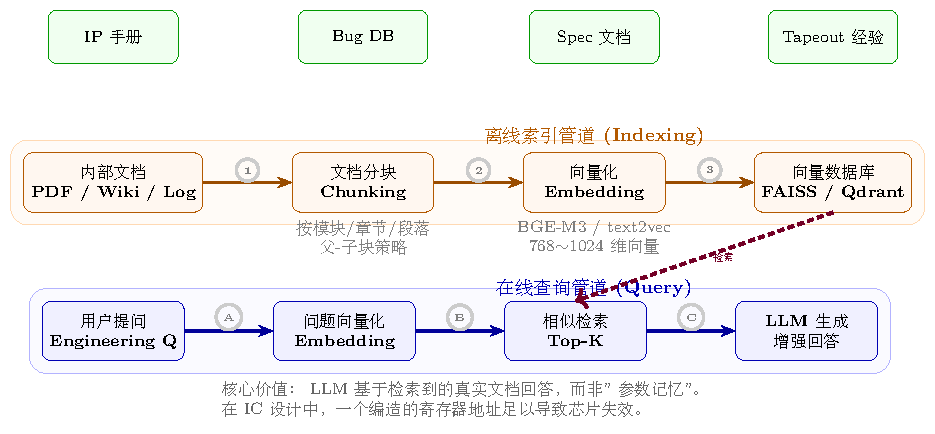
\includegraphics[width=0.95\textwidth]{figures/06-rag-pipeline.pdf}
\caption{RAG 工作流管道：上半部分为离线索引（文档→分块→Embedding→向量库），下半部分为在线查询（问题→检索→LLM 生成），两者通过向量数据库连接。}
\end{figure}

\subsubsection{Embedding 的本质}

Embedding 是将文本映射到高维向量空间的过程。"语义相近"的文本在这个空间中距离近，"语义无关"的文本距离远。

对于技术文档：
\begin{itemize}
    \item "时钟域交叉"和"CDC"会被映射到相近的向量
    \item "Bandgap 温度系数"和"TC"会被映射到相近的向量
    \item "set\_false\_path"和"时序例外"会被映射到相近的向量
\end{itemize}

Embedding 模型的质量直接影响 RAG 的检索质量。对于中英文混合的 IC 文档，推荐使用多语言 Embedding 模型如 BGE-M3 或 text2vec-large-chinese。

\subsubsection{Chunking 为什么重要}

Chunking 是 RAG 中最被低估的环节。分块策略直接影响检索质量。

\textbf{IC 文档的特殊挑战}：
\begin{itemize}
    \item Verilog 代码块不应该被切断（破坏了语法完整性）
    \item 寄存器表（多列表格）需要特殊处理
    \item 时序图/波形图的文字描述需要保持连贯
    \item 数学公式不能在中途截断
\end{itemize}

\textbf{推荐策略}：
\begin{itemize}
    \item 对于代码文档：按函数/模块边界分块
    \item 对于 Spec 文档：按章节分块，保留层级结构
    \item 对于技术笔记：按段落分块，保持语义完整
    \item 使用"父子块"（Parent-Child Chunking）：检索小粒度块，返回大粒度块
\end{itemize}

\subsubsection{向量数据库方案对比}

\begin{table}[htbp]
\centering
\caption{向量数据库方案对比}
\begin{tabular}{p{2.5cm}p{4cm}p{4.5cm}p{1cm}p{1cm}}
\hline
\textbf{方案} & \textbf{适合场景} & \textbf{部署复杂度} & \textbf{性能} & \textbf{社区} \\
\hline
FAISS (Meta) & 研究/PoC，单机 & 低（Python 库）& 极高 & 活跃 \\
Chroma & 小团队 PoC & 极低 & 中等 & 活跃 \\
Milvus & 企业生产 & 中高（需要 etcd/MinIO）& 高 & 活跃 \\
Qdrant & 企业生产 & 中（Rust 实现，单二进制）& 高 & 活跃 \\
pgvector & 已有 PostgreSQL 的团队 & 低（PostgreSQL 插件）& 中等 & 活跃 \\
Elasticsearch & 已有 ES 的团队 & 低（已有基础设施）& 中等 & 成熟 \\
\hline
\end{tabular}
\end{table}

\textbf{对初创 IC 公司的推荐}：

PoC 阶段：Chroma（嵌入式，零运维）或 FAISS（性能最好，纯 Python）。

生产阶段：Qdrant（单二进制部署，高性能，运维简单）或 pgvector（如果已有 PostgreSQL）。

不推荐 Milvus 给初创——它需要 etcd + MinIO + Pulsar 等依赖，运维负担太重。

% ======================================================================
% 第五章：Agent 在 IC 设计中的可能性
% ======================================================================

\section{Agent 在 IC 设计中的可能性}

\subsection{什么是 AI Agent}

AI Agent = LLM + 工具调用（Tool Calling）+ 规划（Planning）+ 记忆（Memory）+ 执行循环。

一个典型的 Agent 工作流：
\begin{enumerate}
    \item 用户给出目标（如"分析这个仿真 log 中的 warning"）
    \item Agent 规划步骤（读取 log $\rightarrow$ 分类 warning $\rightarrow$ 查询内部知识库 $\rightarrow$ 生成报告）
    \item Agent 调用工具（读文件、查数据库、运行脚本）
    \item Agent 根据工具返回结果调整计划
    \item 循环直到完成目标
\end{enumerate}

\begin{figure}[htbp]
\centering
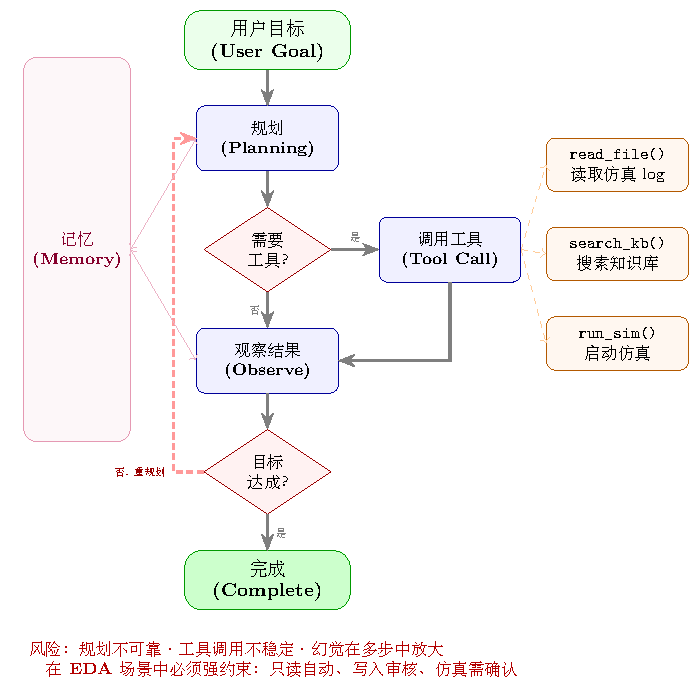
\includegraphics[width=0.85\textwidth]{figures/07-agent-loop.pdf}
\caption{AI Agent 执行循环：用户目标→规划→工具调用→观察→判断→重规划或完成。左侧 Memory 组件提供跨步骤上下文记忆。}
\end{figure}

\subsection{当前 Agent 的核心能力}

\subsubsection{Tool Calling / Function Calling}

LLM 可以"决定"调用哪个工具（函数/API），并生成调用参数。例如：
\begin{itemize}
    \item 调用 `read\_file(path)` 读取仿真 log
    \item 调用 `search\_knowledge\_base(query)` 搜索内部文档
    \item 调用 `run\_simulation(config)` 启动仿真
\end{itemize}

这是 Agent 的基础能力，当前已比较成熟（OpenAI、Anthropic、开源模型都支持）。

\subsubsection{MCP（Model Context Protocol）}

Anthropic 提出的标准化协议，让 LLM 通过统一接口连接各种工具和数据源。类比：MCP 之于 AI Agent，就像 USB-C 之于外设——一个标准接口。

对于 IC 公司：可以开发 MCP Server 封装 EDA 工具（如启动仿真、读取波形、查询 PDK），然后任何支持 MCP 的 Agent 都可以调用。

\subsubsection{Workflow Engine}

Workflow Engine（如 LangGraph、Prefect、Temporal）用于定义多步骤的 Agent 流程，支持条件分支、并行执行、错误重试、人工审核节点。

在 IC 场景中：一个典型的 regression 分析 workflow 可能包含：自动运行仿真 $\rightarrow$ 收集 log $\rightarrow$ 分类 FAIL/PASS $\rightarrow$ 对 FAIL 案例做根因分析 $\rightarrow$ 生成报告 $\rightarrow$ 发送通知。

\subsection{为什么当前 Agent 很容易失控}

这是 Agent 在 IC 设计中最核心的风险：

\begin{enumerate}
    \item \textbf{规划不可靠}：LLM 的"推理"本质是概率性的 token 预测，不是真正的逻辑推理。在复杂的 IC 设计场景中，Agent 可能规划出"看起来合理但实际上错误"的步骤
    \item \textbf{工具调用不稳定}：LLM 可能用错误的参数调用工具，或者遗漏关键步骤
    \item \textbf{幻觉放大}：Agent 的多步骤执行中，每一步都可能引入幻觉，错误会累积
    \item \textbf{缺乏领域知识}：LLM 不知道什么是"危险的 EDA 操作"——比如不小心覆盖了重要的仿真结果
    \item \textbf{无成本意识}：LLM 可能反复启动昂贵的仿真而不自知
\end{enumerate}

\subsection{EDA 场景需要强约束}

在 EDA 场景中，一个错误可能导致：
\begin{itemize}
    \item 仿真结果被覆盖（丢失数天的计算）
    \item 错误的约束导致综合结果异常
    \item 错误的 tapeout 数据——这是灾难性的
\end{itemize}

\textbf{因此，Agent 在 EDA 中必须是"受控的"}：

\begin{itemize}
    \item \textbf{只读操作可以自动化}：读 log、读报告、读波形摘要、搜索文档
    \item \textbf{写入操作需要人工审核}：修改 constraint、修改 RTL、提交代码
    \item \textbf{仿真启动需要确认}：确认参数正确、确认不会覆盖已有结果
    \item \textbf{所有操作必须有审计日志}
\end{itemize}

\begin{figure}[htbp]
\centering
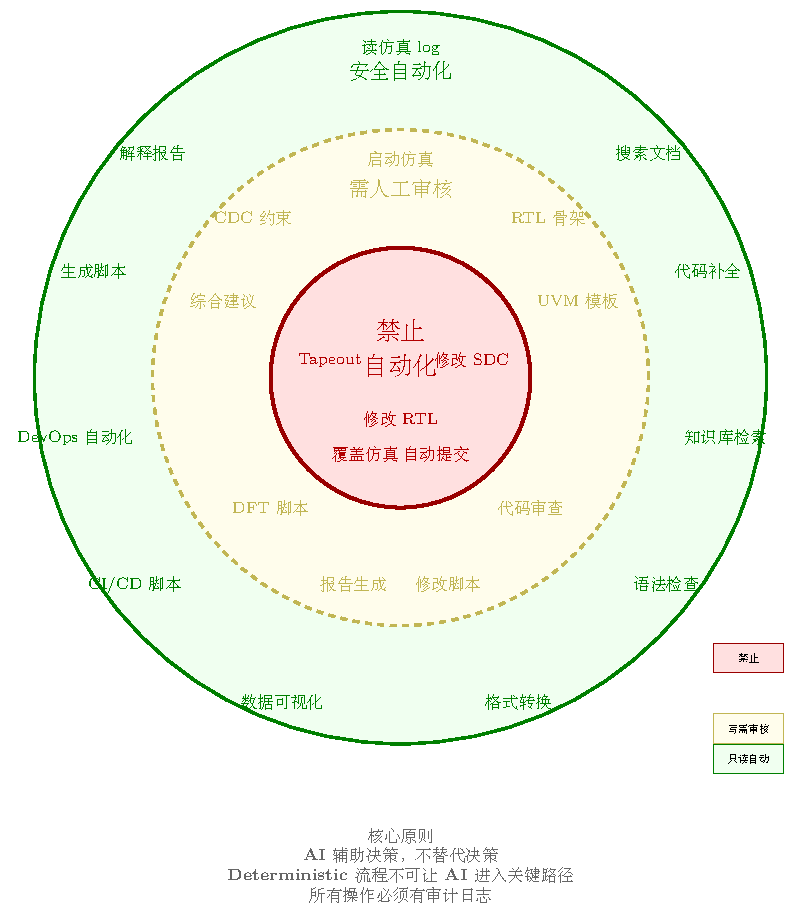
\includegraphics[width=0.85\textwidth]{figures/08-agent-safety-boundary.pdf}
\caption{EDA Agent 安全边界模型：绿圈=只读自动化（安全），黄圈=写入需人工审核，红圈=禁止自动化。核心原则：AI 辅助决策而非替代决策。}
\end{figure}

\subsection{Deterministic Workflow 的重要性}

\textbf{核心原则：AI 应该辅助决策，而不是替代决策。}

在 IC 设计中，很多流程本质上应该是 deterministic（确定性的）：
\begin{itemize}
    \item 仿真 regression 的 PASS/FAIL 判定——确定性
    \item Coverage 数据的收集——确定性
    \item Timing report 的提取——确定性
    \item Lint/CDC 检查——确定性
\end{itemize}

AI 的价值在于：
\begin{itemize}
    \item 在执行确定性流程之前，帮助规划（"应该跑哪些 corner？"）
    \item 在执行确定性流程之后，帮助分析（"为什么这些 case FAIL 了？"）
    \item 在确定性流程之间，做智能编排（"覆盖率不够，自动建议增加哪些测试"）
\end{itemize}

\textbf{不要把 AI 放在确定性流程的"关键路径"上。} 这是工程实践的铁律。

\subsection{当前可行的 Agent 应用场景}

\begin{itemize}
    \item \textbf{仿真 Log 分析 Agent}：自动读取 regression log，分类错误类型，给出初步分析 → 低风险，高收益
    \item \textbf{文档问答 Agent}：RAG + Agent，搜索内部文档回答技术问题 → 低风险，高收益
    \item \textbf{代码审查 Agent}：读取 PR diff，对照 coding guideline 提出建议 → 中风险，中收益
    \item \textbf{仿真报告生成 Agent}：自动收集结果、画图、生成 summary → 低风险，高收益
\end{itemize}

\textbf{当前不适合的 Agent 场景}：
\begin{itemize}
    \item 自动修改 RTL（风险太高）
    \item 自动修改 constraint（风险太高）
    \item 自动决定 tapeout 参数（绝对不行）
\end{itemize}

% ======================================================================
% 第六章：现实可落地的建议方案
% ======================================================================

\section{最终建议方案}

\subsection{方案 A：最低成本 PoC 方案（¥25K--¥35K）}

\begin{table}[htbp]
\centering
\caption{方案 A：最低成本 PoC}
\begin{tabular}{p{2cm}p{7cm}}
\hline
\textbf{组件} & \textbf{配置} \\
\hline
GPU & 1$\times$ RTX 4090 24GB（约 ¥13K）\\
CPU & AMD Ryzen 9 7950X 或 Intel i9-14900K \\
RAM & 64GB DDR5（约 ¥2K）\\
存储 & 2TB NVMe SSD（约 ¥1K）\\
主板 & X670/B650 或 Z790（约 ¥2K）\\
电源 & 1000W 80+ Gold（约 ¥1K）\\
机箱/散热 & 约 ¥1K \\
OS & Ubuntu 24.04 LTS \\
推理框架 & vLLM（生产级）+ Ollama（备用）\\
模型 & Qwen2.5-Coder-14B-Q4 / 32B-Q4 \\
RAG & Chroma + BGE-M3 Embedding \\
Web UI & Open WebUI \\
监控 & nvitop + Prometheus + Grafana（可选）\\
\hline
\textbf{总硬件成本} & \textbf{约 ¥20K--¥25K（不含显示器）} \\
\textbf{月电费} & 约 ¥200--¥300（按每天 12 小时使用）\\
\hline
\end{tabular}
\end{table}

\textbf{能力}：
\begin{itemize}
    \item 3--8 人同时使用
    \item 32K 上下文
    \item 代码补全、代码审查、文档问答
    \item 小型 RAG 知识库（100--1000 份文档）
    \item 响应速度：20--50 tok/s（单用户），10--20 tok/s（3 用户并发）
\end{itemize}

\textbf{风险}：
\begin{itemize}
    \item 单卡无冗余，GPU 故障则服务中断
    \item 24GB 显存限制了模型选择（32B Q4 是上限）
    \item 消费级显卡的散热和稳定性不如企业级
    \item 无 ECC，极低概率的内存错误可能导致输出异常
\end{itemize}

\subsection{方案 B：初创公司推荐方案（¥60K--¥100K）}

\begin{table}[htbp]
\centering
\caption{方案 B：初创公司推荐方案}
\begin{tabular}{p{2cm}p{11cm}}
\hline
\textbf{组件} & \textbf{配置} \\
\hline
GPU & 2$\times$ RTX 4090 24GB 或 1$\times$ RTX 5090 32GB \\
CPU & AMD Threadripper 或 Intel Xeon W \\
RAM & 128GB DDR5 \\
存储 & 4TB NVMe（系统） + 8TB HDD/SSD（数据备份）\\
网络 & 千兆以太网（已有局域网即可）\\
OS & Ubuntu 24.04 LTS \\
推理框架 & vLLM（张量并行）+ SGLang（结构化输出）\\
模型 & Qwen2.5-Coder-32B-Q4\_K\_M（主力）/ Qwen2.5-72B-Q4（高级任务）\\
RAG & Qdrant + BGE-M3 或 text2vec-large-chinese \\
Web UI & Open WebUI + Continue.dev（IDE 插件）\\
Agent & LangChain/LangGraph（实验性）\\
监控 & nvitop + Prometheus + Grafana + Loki（日志）\\
备份 & restic + 异地备份（NAS 或云存储）\\
\hline
\textbf{总硬件成本} & \textbf{约 ¥40K--¥60K（双 4090）/ ¥50K--¥70K（RTX 5090）} \\
\textbf{月电费} & 约 ¥400--¥600（24/7 运行）\\
\hline
\end{tabular}
\end{table}

\textbf{能力}：
\begin{itemize}
    \item 10--20 人同时使用
    \item 64K--128K 上下文（RTX 5090 32GB 优势明显）
    \item 完整 RAG 系统（内部文档、IP 手册、Bug DB）
    \item 代码补全 + 代码审查 + 文档问答 + 脚本生成
    \item Agent 原型（仿真 log 分析、自动报告生成）
    \item OpenAI API 兼容，可对接各种工具
\end{itemize}

\textbf{为什么不要 Kubernetes}：

对初创 IC 公司来说，K8s 是过度设计：
\begin{itemize}
    \item 你们只有 1--2 台 GPU 服务器，不需要容器编排
    \item K8s 的 GPU 支持（NVIDIA Device Plugin、GPU Operator）增加运维负担
    \item Docker Compose 或 systemd 足以管理 2--3 个服务
    \item 当团队超过 50 人、GPU 超过 4 张时再考虑 K8s
\end{itemize}

\textbf{为什么不要 InfiniBand / NVLink}：

对初创公司，InfiniBand 和 NVLink 不是必需的：
\begin{itemize}
    \item RTX 4090 不支持 NVLink，多卡通信走 PCIe 4.0（约 32 GB/s）
    \item 张量并行在小规模（2--4 卡）下，PCIe 带宽足够
    \item InfiniBand 只有在大规模集群（8+ 节点）时才需要
    \item 你们的并发量和模型规模不需要这些
\end{itemize}

\subsection{方案 C：长期企业化演进方案（未来 1--3 年）}

当公司规模增长（50+ 工程师，模型需求升级），考虑以下演进路径：

\textbf{Phase 1（当前--6 个月）}：方案 B，单机双卡，积累使用数据

\textbf{Phase 2（6--18 个月）}：
\begin{itemize}
    \item 升级到企业级 GPU（A100 80GB 或 H100），通过云租用或购买
    \item 部署专业的模型管理平台（如 Harbor + MLflow）
    \item 建立完善的 RAG 知识库（全公司文档纳入）
    \item 引入微调能力（LoRA/QLoRA fine-tuning on IC domain data）
    \item Agent 在非关键路径上正式使用（log 分析、报告生成）
\end{itemize}

\textbf{Phase 3（18--36 个月）}：
\begin{itemize}
    \item 多节点部署（2--4 台 GPU 服务器）+ 负载均衡
    \item K8s + GPU Operator（此时才需要）
    \item 多模型服务（代码模型 + 通用模型 + Embedding 模型分不同实例）
    \item 与 EDA 流程深度集成（CI/CD 中嵌入 LLM 审查步骤）
    \item 自定义 IC 领域模型微调（在开源代码模型上做 domain adaptation）
\end{itemize}

\begin{figure}[htbp]
\centering
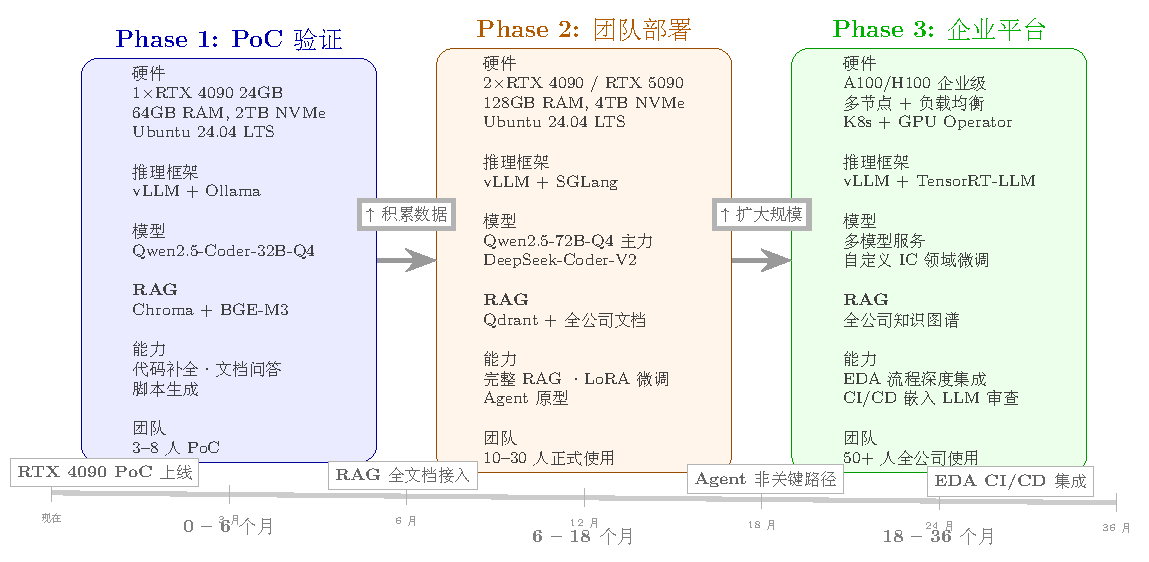
\includegraphics[width=0.95\textwidth]{figures/09-evolution-roadmap.pdf}
\caption{LLM 部署三阶段演进路线：Phase 1 (0--6月) PoC 单卡验证 → Phase 2 (6--18月) 团队正式部署 RAG+Agent → Phase 3 (18--36月) 企业平台多节点多模型。}
\end{figure}

\subsection{关键决策：买硬件 vs. 用云}

\begin{table}[htbp]
\centering
\caption{自建 vs 云 GPU 对比（以 RTX 4090 24GB 为例）}
\begin{tabular}{p{3cm}p{3.5cm}p{4.5cm}}
\hline
\textbf{维度} & \textbf{自建（RTX 4090）} & \textbf{云 GPU（A10/4090 等效）} \\
\hline
硬件成本 & ¥13K（一次性）& ¥0 \\
月费 & ¥300（电费）& ¥5K--¥8K（24/7）\\
回本周期 & — & 2--3 个月 \\
数据安全 & 完全本地 & 需评估（VPC 内可接受）\\
运维 & 需要 Linux 基础 & 运维由云厂商负责 \\
扩展性 & 有限（加卡即可）& 弹性 \\
适用场景 & 长期使用、数据敏感 & 短期 PoC、弹性需求 \\
\hline
\end{tabular}
\end{table}

\textbf{建议}：对于初创 IC 公司，\textbf{自建方案在 3 个月内回本}。IC 公司的代码和数据是核心资产，本地部署在安全性和长期成本上都有优势。如果只是 1--2 周的 PoC 验证，云 GPU 更灵活。

\subsection{哪些方向最值得投入（优先级排序）}

\begin{enumerate}
    \item \textbf{RAG 知识库建设}（最高优先级，即刻开始）

    这是投入产出比最高的方向。整理内部文档、IP 手册、设计规范、Tapeout 经验，建立结构化的知识库。即使 LLM 本身能力有限，一个良好的知识库也有独立价值。

    \item \textbf{代码补全（IDE 集成）}（高优先级）

    Continue.dev + 本地模型，提供 Verilog/V/SV/Python 的代码补全。这是工程师每天都能感受到的提效。

    \item \textbf{UVM/验证自动化}（高优先级）

    自动生成 UVM 模板、SVA、coverage model。验证代码量大且模式化，LLM 在此场景收益显著。

    \item \textbf{仿真脚本/DevOps 自动化}（高优先级）

    Python/Shell/Tcl/Makefile 生成，CI/CD pipeline 编写。安全、高效、通用。

    \item \textbf{Agent（log 分析/报告生成）}（中优先级）

    在非关键路径上实验 Agent。先从仿真 log 自动分析和回归报告生成开始。

    \item \textbf{微调（Fine-tuning）}（中低优先级）

    在积累足够多的 IC 领域数据后再考虑。现阶段先用 RAG 解决"领域知识"问题。

    \item \textbf{RTL 自动生成}（低优先级，高风险）

    当前不推荐。RTL 质量要求太高，LLM 的幻觉风险太大。只在有经验的工程师严格审查下使用。
\end{enumerate}

\begin{figure}[htbp]
\centering
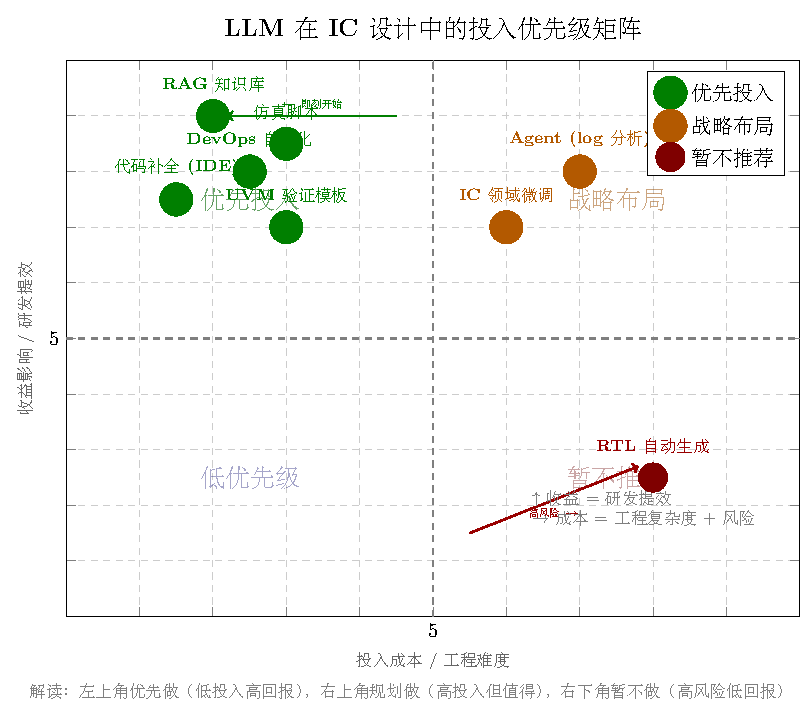
\includegraphics[width=0.85\textwidth]{figures/10-priority-matrix.pdf}
\caption{LLM 在 IC 设计中的投入优先级矩阵：横轴为投入成本/工程难度，纵轴为研发提效收益。左上角优先做、右上角规划做、右下角暂不做。}
\end{figure}

\subsection{哪些方向现在只是"AI 幻觉"}

\begin{itemize}
    \item \textbf{"AI 自动设计芯片"}——这是科幻，不是工程。芯片设计涉及大量物理约束、工艺特性、多物理场仿真，LLM 无法替代这些
    \item \textbf{"AI 替代 SPICE 仿真"}——不可能。SPICE 解的是微分方程，LLM 做的是概率性 token 预测，本质完全不同
    \item \textbf{"AI 自动发现新电路拓扑"}——目前没有可信的证据表明 LLM 能创新电路设计
    \item \textbf{"AI 替代资深工程师"}——不会。AI 是工具，放大的是工程师的能力，不是替代工程师的判断
\end{itemize}

\subsection{未来 3--5 年可能成熟的能力}

\begin{itemize}
    \item \textbf{多模态 EDA AI}：能"看懂"电路图、波形图、Layout 的视觉-语言模型
    \item \textbf{EDA 专用代码模型}：在 Verilog/V/SV/UVM 上深度训练的代码模型，理解时序、面积、功耗约束
    \item \textbf{可信任的 EDA Agent}：在确定性工作流框架下的 Agent，能在安全边界内自动执行设计空间探索
    \item \textbf{AI 辅助的模拟电路优化}：结合 SPICE 仿真和 AI 的电路参数自动优化（类似 Bayesian Optimization + LLM）
\end{itemize}

\subsection{对 IC 公司而言，最关键的竞争壁垒到底是什么}

\begin{center}
\fbox{
\begin{minipage}{0.9\textwidth}
\textbf{结论：AI 不是壁垒。你的电路设计能力、IP 积累、工程师经验、内部知识体系才是壁垒。}

AI 是一个 force multiplier——它让强者更强，但它不能让弱者变成强者。

一家没有深厚设计积累的公司，用了 AI 也不会突然设计出好的 SerDes。
一家有深厚积累的公司，用了 AI 可以让资深工程师的效率翻倍。

\textbf{所以：把 AI 当作效率工具来投资，而不是当作核心壁垒来依赖。}
\end{minipage}
}
\end{center}

\subsection{最后的话}

作为同时了解 AI Infra 和 IC 设计流程的人，我的核心建议是：

\begin{enumerate}
    \item \textbf{先花 ¥25K 做 PoC}。买一张 RTX 4090，装 Ubuntu，部署 vLLM + Qwen2.5-Coder-32B + Open WebUI。让 3--5 个工程师用一个月，收集反馈。
    \item \textbf{如果反馈正面}，升级到方案 B（双卡或 RTX 5090），同时开始建设 RAG 知识库。
    \item \textbf{如果反馈负面}，¥25K 的显卡可以给工程师当深度学习工作站用，不会浪费。
    \item \textbf{不要在 PoC 之前就规划"企业级 AI 平台"}——过度设计是初创公司最常见的错误。
    \item \textbf{不要低估"整理内部文档"的价值}——这不仅是给 AI 用的，对新人培训、知识传承、设计复用都有巨大价值。
    \item \textbf{AI 是 2026 年的基础设施}——就像 2010 年的 Git、2015 年的 CI/CD。早投入、早受益，但不要期待奇迹。
\end{enumerate}

\vspace{1em}
\begin{center}
\rule{0.5\textwidth}{0.4pt}

\textit{文档版本：v1.0 — 2026-05-17}

\textit{适用对象：初创 IC 设计公司技术决策者}

\textit{本文档中的硬件价格和模型性能基于 2026 年 5 月的市场情况，请以实际采购时的行情为准。}
\end{center}

\end{document}
